\documentclass{article}
\usepackage{graphicx}
\usepackage{geometry}
\usepackage{amsmath}
\usepackage{caption} 
\usepackage{float}

\begin{document}

\section*{Question 1}

\subsection*{1.a}

We have that:

\[
P(ALQ_{i} \mbox{is missing}|ALQ_{i}=Yes)=0.3
\]

By definition of the MCAR, it has to be the case that:

\[
P(ALQ_{i} \mbox{is missing}|ALQ_{i}=Yes)=P(ALQ_{i} \mbox{is missing}),
\]

and:

\[
P(ALQ_{i} \mbox{is missing}|ALQ_{i}=No)=P(ALQ_{i} \mbox{is missing}),
\]

$\forall$ \textit{i}

Thus:
\[
P(ALQ_{i} \mbox{is missing}|ALQ_{i}=No)=P(ALQ_{i} \mbox{is missing}|ALQ_{i}=Yes)=0.3,
\]

so the answer choice is (\textit{ii}).

\subsection*{1.b}

By definition of the MAR, it has to be the case that:

\[
P(ALQ_{i} \mbox{is missing}|ALQ,\mbox{gender})=P(ALQ_{i} \mbox{is missing}|\mbox{gender}),
\]

$\forall$ \textit{i}

Thus, the answer choice is (\textit{ii}).

\subsection*{1.c}

The information given is not sufficient to determine $P(ALQ_{i} \mbox{is missing}|Female)$. 

Thus, the answer choice is (\textit{iii}).

\section*{Question 2}

Arrange the data set into 100 rows and 10 columns. Let \textit{i} be a row index and \textit{j} be a column index.

Define  $x_{i,j}=\emptyset$ if  $(i,j)^{th}$ element of the data matrix is missing and $x_{i,j}{\ne}\emptyset$ otherwise. Furthermore, let:

\[
I_{i}=
\begin{cases}
1 & \textit{if $\cap^{10}_{j=1}x_{i,j}{\ne}\emptyset$}\\
0 & \textit{otherwise}
\end{cases}
\]

Under a complete case analysis any row with at least one observation missing is deleted. Thus, the total number of observations in the subsample used under a complete case analysis is:

\[
C=10\sum^{100}_{i=1}I_{i}
\] 

Note that $I_{i}=0$ whenever $x_{i,j}=\emptyset$ for at least one \textit{j} for a given \textit{i}. Additionally, note that C is maximized when there are as few of $i^{th}$ for which  $I_{i}=0$ as possible and is minimized when there are as many of $i^{th}$ for which  $I_{i}=0$ as possible. Or, given the definition of $I_{i}$, C is maximized if $x_{i,j}=\emptyset$ is present in as few rows as possible and is minimized if $x_{i,j}=\emptyset$ is present in as many rows as possible. Given that we have 10 observations missing for each \textit{j=1,...,10} there is a total of 100 missing observations. Thus, C is maximized if 10 rows contain only missing observations and is minimized if 100 rows contain a missing observation:
Let $i^{'}+1:i^{'}+10$ be indexes of the rows with all elements missing, then:
\[
C_{max}=10\left(\sum^{i^{'}}_{i=1}I_{i}+\sum^{i^{'}+10}_{i=i^{'}+1}I_{i}+\sum^{100}_{i=i^{'}+11}I_{i}\right)=10\left(\sum^{i^{'}}_{i=1}I_{i}+\sum^{100}_{i=i^{'}+11}I_{i}\right)=10(i^{'}-1+1+100-i^{'}-11+1)=900;
\]  

And:

\[
C_{min}=10\left(\sum^{100}_{i=1}I_{i}(\cap^{10}_{j=1}x_{i,j}=\emptyset)\right)=10\left(\sum^{100}_{i=1}0\right)=0;
\]  

\section*{Question 3}

We have the following data generating process:

\begin{equation}\label{Eq_1}\begin{array}{c}
Y_{1,i}=1+Z_{1,i}\\
Y_{2,i}=5+2Z_{1,i}+Z_{2,i},
\end{array}\end{equation}

with:

\[
\begin{pmatrix}
Z_{1,i} \\
Z_{2,i} \\
Z_{3,i}
\end{pmatrix}{\sim}N\left(\begin{pmatrix}
0 \\
0 \\
0
\end{pmatrix}, \begin{pmatrix}
1 & 0 & 0 \\
0 & 1 & 0 \\
0 & 0 & 1
\end{pmatrix}\right)
\]

$\forall$ \textit{i}.

Furthermore, $Y_{2,i}$ is missing if:

\[
a\left(Y_{1,i}-1\right)+b\left(Y_{2,i}-5\right)+Z_{3,i}<0,
\]

for some constants a and b.

\subsection*{3.a}

With a=2 and b=0 $Y_{2,i}$ the missingness criterion becomes:

\[
2\left(Y_{1,i}-1\right)+Z_{3,i}<0.
\]

Note that since both $Y_{1,i}$ and $Y_{2,i}$ are independent of $Z_{3,i}$ $\forall$ \textit{i} and given the above missingness criterion:

\[
P\left(Y_{2,i} \mbox{is missing}|Y_{1,i},Y_{2,i}\right)=P\left(Y_{2,i} \mbox{is missing}|Y_{1,i}\right),
\]

$\forall$ \textit{i}, which is the condition defining the MAR mechanism.


The marginal distributions of complete and observed $Y_{2}$ are presented in Figure (\ref{Fig_1}).

\begin{figure}[h]
\centering
\caption{Complete and observed marginal distributions of $Y_{2}$}
\label{Fig_1}
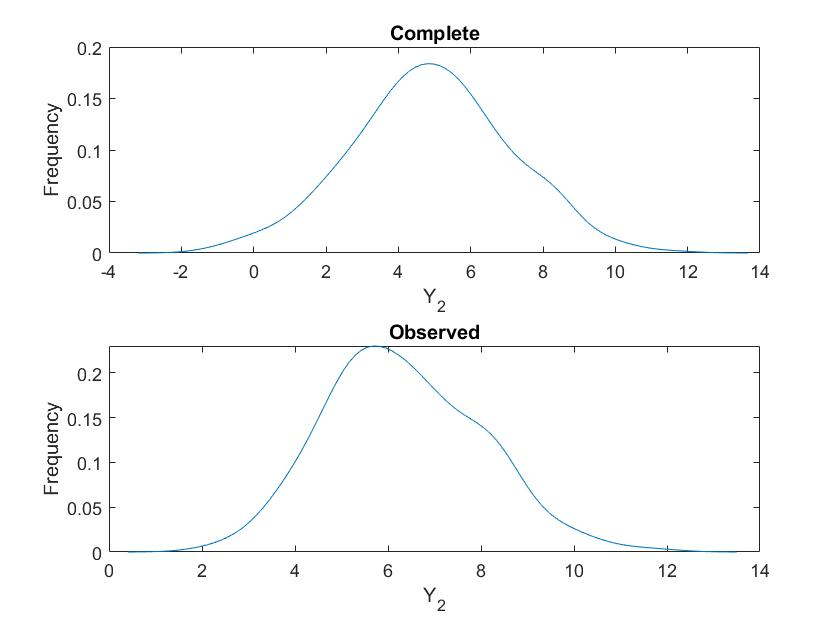
\includegraphics[width=8cm]{q3a.jpg}
\end{figure} 

Note that $Y_{2}$ and $Y_{1}$ are not independent. Thus, the distribution of $Y_{2}$ conditional on $Y_{1}$ does not equal to the marginal distribution of $Y_{2}$. Under the complete data, in order to obtain the marginal distribution of $Y_{2}$, we integrate over all possible values of $Y_{1}$. Thus this marginal distribution does not depend on a realization of $Y_{1}$. However, in the case of the 'observed' data, we integrate over only a subset of possible values of $Y_{1}$. Thus, the 'marginal' distribution of observed $Y_{2}$ still depends on realizations of $Y_{1}$.  The difference between the marginal distribution and the conditional one is reflected as the difference in the empirical distributions of $Y_{2}$ in the complete and the observed cases. 

\subsection*{3.b}

The marginal distribution of the complete data and the one obtained from the stochastic regression imputation method are presented in the Figure  (\ref{Fig_2}).

\begin{figure}[H]
\centering
\caption{Complete and imputed marginal distributions of $Y_{2}$}
\label{Fig_2}
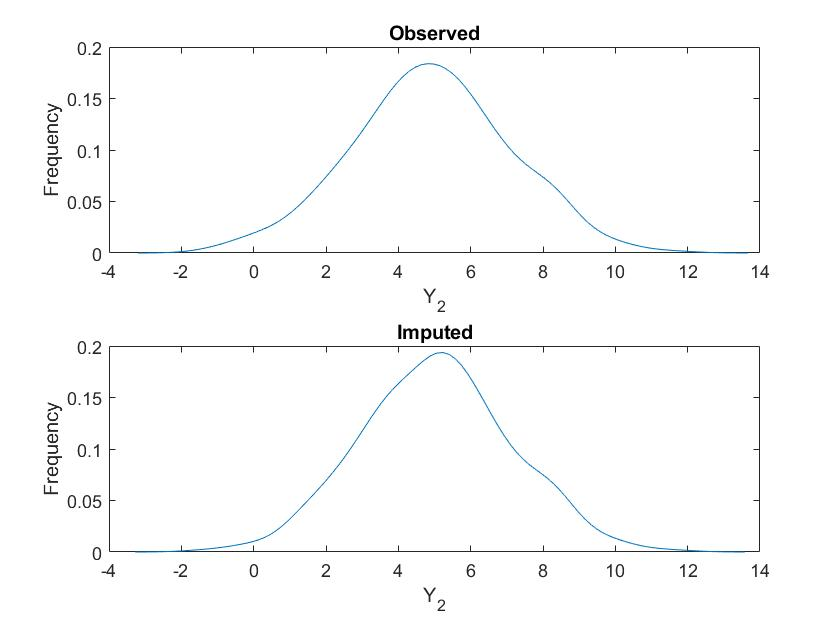
\includegraphics[width=8cm]{q3b.jpg}
\end{figure} 

Note the similarity between the distributions. While fitting the regression we estimate $E\left[Y_{2,i}|Y_{1,i}\right]$. The distribution of the missing values is then obtained by adding the error to the estimate of this conditional mean. The error is drawn from a Normal distribution with the empirical variance covariance matrix obtained from fitting the regression. The similarity of the distributions of complete and completed by the imputation data indicates that, the imputation gives a good approximation to the conditional distribution of $Y_{2}$ given $Y_{1}$. 


\subsection*{3.c}

With a=0 and b=2 $Y_{2,i}$ the missingness criterion becomes:

\[
2\left(Y_{2,i}-5\right)+Z_{3,i}<0.
\]

Given that $Y_{1,i}$ and $Y_{2,i}$ are independent of $Z_{3,i}$ $\forall$ \textit{i} the missingness criterion implies that:

\[
P\left(Y_{2,i} \mbox{is missing}|Y_{1,i},Y_{2,i}\right)=P\left(Y_{2,i} \mbox{is missing}|Y_{2,i}\right),
\]

$\forall$ \textit{i}, which is the condition defining the MNAR mechanism.

The marginal distributions of complete and observed $Y_{2}$ are presented in Figure (\ref{Fig_3}).

\begin{figure}[H]
\centering
\caption{Complete and observed marginal distributions of $Y_{2}$}
\label{Fig_3}
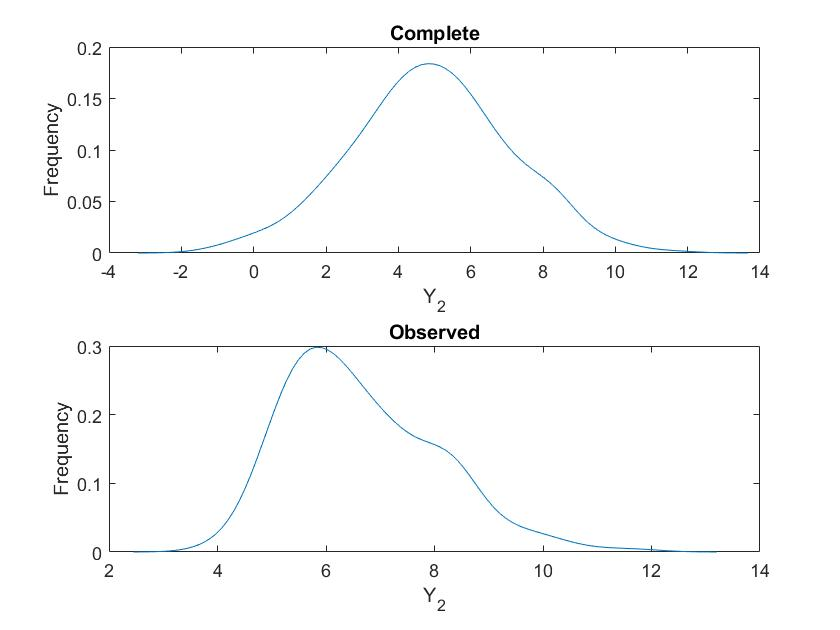
\includegraphics[width=8cm]{q3c.jpg}
\end{figure} 

The distributions are visibly different. The observed distribution is a truncated distribution, that is it is a distribution of $Y_{2}$  conditional on  $Y_{2,i}>-\frac{Z_{3,i}}{2}+5$. The missingness condition implies that many negative realizations of the marginal distribution of complete $Y_{2}$ are deleted in the observed data. 

Note that the difference between the complete and the observed case is more pronounced in the Figure (\ref{Fig_3}) than in the Figure (\ref{Fig_1}). A glance at the the Eq.(\ref{Eq_1}) reveals that the relation between $Y_{2}$ and $Y_{1}$ is noisy because of the presence of $Z_{2}$. Thus, missingness conditional on $Y_{1}$ is closer to the MCAR case than missingness conditional on $Y_{2}$. Given this observation, the differences between the complete and the observed case should indeed be less pronounced in the case of missigness conditional on $Y_{1}$ than in the case of missingness conditional on $Y_{2}$. This is what is observed in the Figure (\ref{Fig_1}) and in the Figure (\ref{Fig_3}).    

\subsection*{3.d}

  
The marginal distribution of the complete data and the one obtained from the stochastic regression imputation method are presented in the Figure  (\ref{Fig_4}).

\begin{figure}[H]
\centering
\caption{Complete and imputed marginal distributions of $Y_{2}$}
\label{Fig_4}
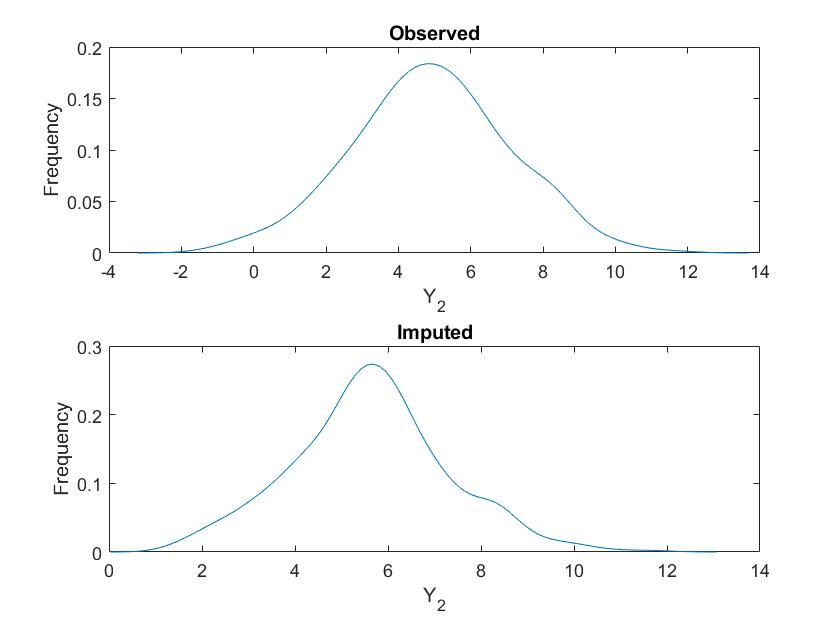
\includegraphics[width=8cm]{q3d.jpg}
\end{figure} 

While fitting the regression we estimate $E\left[Y_{2,i}|Y_{1,i}\right]$. After adding an error term that has Normal distribution with the empirical variance-covariance matrix, the resulting data should approximate the distribution of $Y_{2,i}$ conditional on   $Y_{2,i}<-\frac{Z_{3,i}}{2}+5$. It is visible from the graphs that this approximation is very rough. 

\section*{Question 4}


\subsection*{4.a}

Only the recovery time has missing observations. Removing the rows corresponding to these three missing observations leaves 22 observations on each variable. The required information about basic statistics is presented in Table (\ref{Tab_1}).


\begin{table}[H]
\caption{Basic statistics for the recovery time: complete case analysis}
\label{Tab_1}
\begin{tabular}{|c |c| c|}

\hline
\hline
 \textbf{Number of observations} & \textbf{Mean} &\textbf{SE(Mean)} \\[2ex]
\hline
22 &19.2727 & 2.6030 \\
\hline
 &\textbf{CORR with the log-dose} &\textbf{CORR with the blood pressure} \\[2ex] 
\hline
 &0.2391 &-0.0195 \\
\hline
\hline

\end{tabular}
\end{table}


\subsection*{4.b}

Under the mean imputation, we substitute the missing values by the mean of the non-missing values. The values of the basic statistics after the mean imputation are presented in Table (\ref{Tab_2}).

\begin{table}[H]
\caption{Basic statistics for the recovery time: mean imputation}
\label{Tab_2}
\begin{tabular}{|c |c| c|}

\hline
\hline
 \textbf{Number of observations} & \textbf{Mean} &\textbf{SE(Mean)} \\[2ex]
\hline
25 &19.2727 &2.2841 \\
\hline
 &\textbf{CORR with the log-dose} &\textbf{CORR with the blood pressure} \\[2ex] 
\hline
 &0.2151 &-0.0193 \\
\hline
\hline
 

\end{tabular}
\end{table}


As expected, the mean of the recovery time under the mean imputation equals to the mean recovery time under the complete case analysis. Furthermore, the standard error of the mean and the correlations are lower under the mean imputation than under the complete case analysis.  


\subsection*{4.c}

Under the conditional mean imputation, we substitute the missing values by predictions that result from from fitting a regression of recovery time on a constant, log-dose and blood pressure. The coefficients resulting from running this regression on the complete case data together with the observations on log-dose and blood pressure corresponding to the missing values of the recovery time are then used to fill the missing values. The values of the basic statistics after the conditional mean imputation are presented in Table (\ref{Tab_3}).

\begin{table}[H]
\caption{Basic statistics for the recovery time: conditional mean imputation}
\label{Tab_3}
\begin{tabular}{|c |c| c|}

\hline
\hline
 \textbf{Number of observations} & \textbf{Mean} &\textbf{SE(Mean)} \\[2ex]
\hline
25 &19.4443 &2.3128 \\
\hline
 &\textbf{CORR with the log-dose} &\textbf{CORR with the blood pressure} \\[2ex] 
\hline
 &0.2802 &-0.0111 \\
\hline
\hline
 

\end{tabular}
\end{table}

Note that, since we use two variables for the conditional mean imputation, the pair-wise correlations of the completed data are not necessarily larger than under the complete case analysis. 

\subsection*{4.d}

In the stochastic regression imputation, in addition to the estimated coefficients obtained similarly to the conditional mean imputation method, we also need an estimate of the error variance. We need this variance in order to generate errors that are added to the regression predictions of the missing values. The errors are generated by sampling from the Normal distribution with mean zero and variance set equal to the empirical error variance. Applying stochastic regression imputation to our case leads to the results presented in the Table (\ref{Tab_4}).

Note that we need an extra care while conducting stochastic imputation in this example. This is because the recovery time cannot be negative. Normal distribution has all real line as the support. This implies that some negative error realizations can lead to a negative values imputed into the recovery time data. This possibility can be accounted for by choosing only positive error realizations (thus drawing the observations from a truncated Normal distribution). 


\begin{table}[H]
\caption{Basic statistics for the recovery time: stochastic regression imputation}
\label{Tab_4}
\begin{tabular}{|c |c| c|}

\hline
\hline
 \textbf{Number of observations} & \textbf{Mean} &\textbf{SE(Mean)} \\[2ex]
\hline
25 &18.8114 &2.4670 \\
\hline
 &\textbf{CORR with the log-dose} &\textbf{CORR with the blood pressure} \\[2ex] 
\hline
 &0.3312 &-0.0087 \\
\hline
\hline

\end{tabular}
\end{table}

\subsection*{4.e}

Following the explanation given in the setting, in order to conduct the predictive mean matching, we first need to form a set of predictions for both the observed and the missing values of the recovery time. These predictions can be formed just like in the conditional mean imputation method. Then, prediction of each missing observation of the recovery time is compared to prediction of the non-missing observations of the recovery time and the closest value is selected. The donor is then the observed value of the recovery time that corresponds to the closest prediction.  The results from applying the predictive mean matching to the data are presented in Table (\ref{Tab_5}).


\begin{table}[H]
\caption{Predictive mean matching imputation}
\label{Tab_5}
\begin{tabular}{|c |c| c|}

\hline
\hline
 \textbf{Number of observations} & \textbf{Mean} &\textbf{SE(Mean)} \\[2ex]
\hline
25 &19.4400 &2.4645 \\
\hline
 &\textbf{CORR with the log-dose} &\textbf{CORR with the blood pressure} \\[2ex] 
\hline
 &0.3038 &-0.0321 \\
\hline
\hline

\end{tabular}
\end{table}

\subsection*{4.f}

The predictive mean matching overcomes the problems of the stochastic regression imputation noted in 4.d. Specifically, since the donor is selected from the observed values of the recovery time, the imputed values will not be negative. 

One problem with the predictive mean matching is that it might be the case that the donor is chosen from an incorrect distribution. Take for example the setting of the Question 3.a. If we applied the predictive mean matching in this setting, we would select the donor from $f(Y_{2}|Y_{1}>-\frac{Z_{3}}{2}+1)$ as a substitute to a realization from  $f(Y_{2}|Y_{1}<-\frac{Z_{3}}{2}+1)$. Even a more extreme example is the setting of the Question 3.c where we would choose the donor from $f(y_{2}|Y_{2}>-\frac{Z_{3}}{2}+5)$  as a substitute for the a realization of  $f(y_{2}|Y_{2}<-\frac{Z_{3}}{2}+5)$, thus substituting negative values with the positive ones. 

An additional problem may arise if the fit of the regression that is used in the predictive mean matching is poor. In this case wrong donors can be selected. 




\end{document}